\documentclass[11pt,a4paper]{scrartcl}
\usepackage{gram}
\usetikzlibrary{arrows}
\usetikzlibrary{patterns}
\usepackage{svg}
\usepackage{pgfplots}
\pgfplotsset{compat=1.15}
\usetikzlibrary{arrows}
\pagecolor{fizikawhite}



\title{FIZIKA-2021 Round-1}
\author{FIZIKA Committee}
\date{August 2021}

\begin{document}

\maketitle
 
\vspace{8mm}
\section{Problem 1}
%% INSP Pr 1
\begin{solution}
Magnetic field due to a hollow cylinder will be zero at all interior points and for exterior points hollow cylinder will behave like a wire at the axis. Therefore for the outermost shell at infinity will experience pressure factor of $4$ and due to its own current it will experience a factor of $8$ in pressure expression. Therefore net pressure must be zero in order to make the outermost shell stress free.
$$\frac{\mu_{0} I_{0} I_{\infty}}{4\pi^2 R_{\infty}^2}+\frac{\mu_{0} \left(\frac{I_{0}}{2}\right) I_{\infty}}{4\pi^2 R_{\infty}^2}+\frac{\mu_{0} \left(\frac{I_{0}}{4}\right) I_{\infty}}{4\pi^2 R_{\infty}^2}+\cdots= \frac{\mu_{0} I_{\infty}}{8\pi^2 R_{\infty}^2}$$
$$\mu_{0} I_{0} I_{\infty} \left(1+\frac{1}{2}+\frac{1}{4}+\cdots+\infty\right)=\frac{\mu_{0} I_{\infty}^2}{2}$$
This is a geometric progression with first term 1 and common ratio $1/2$, hence we can write
$$I_{0} \left(\frac{1}{1-\frac{1}{2}}\right)=\frac{I_\infty}{2}$$
$$2I_0 = \frac{I_\infty}{2}$$
$$\boxed{\frac{I_\infty}{I_0}=4}$$
\end{solution}

\section{Problem 2}
\begin{solution}
When $h>1m>x$:\\
We get $$F= mg- v\frac{dm}{dt}$$
$$a= g- \frac{v}{m}\frac{dm}{dt}$$
\begin{equation}
\label{eqn:1}
v \frac{dv}{dx} = g- v\frac{\frac{dm}{dt}}{m}
\end{equation}

Now, Using $\lambda(x)=x$, $$dm = x dx$$
Integrating:
$$m = \frac{x^2}{2}$$
Now substituting in (\ref{eqn:1}), we get:
\end{solution}
\section{Problem 3}
\begin{solution}
Answer: $AC$

Divide the lower rhombus into two equilateral triangles. Let the mutual inductance of a pair of an equilateral triangle having a side (adjacent ones) be '$M_{adj}$' and the ones away be '$M_{away}$'. We need to solve for $M_{adj}+M_{away}$. Dimension analysis helps us realise a triangle of twice the side length has '$2L$' inductance. Taking this as a hint to solve the problem further, we build an extra triangle to the above figure to make it a '$2l$' side equilateral triangle (see the equivalence). \\
\begin{center}
    

\tikzset{every picture/.style={line width=0.75pt}} %set default line width to 0.75pt        

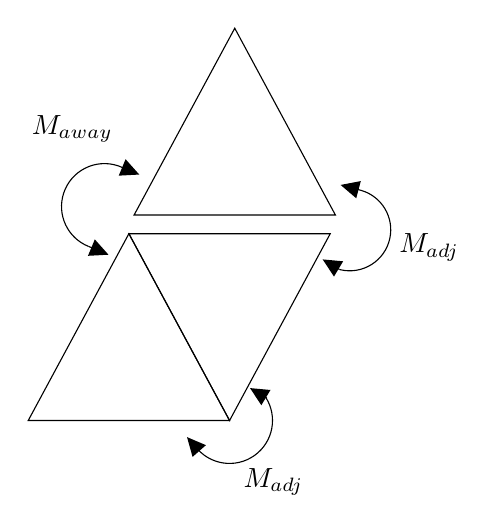
\begin{tikzpicture}[x=0.75pt,y=0.75pt,yscale=-1,xscale=1]
%uncomment if require: \path (0,300); %set diagram left start at 0, and has height of 300

%Shape: Triangle [id:dp45070517116788844] 
\draw   (204,115) -- (252.5,205) -- (155.5,205) -- cycle ;
%Shape: Triangle [id:dp9654711726051111] 
\draw   (252.5,205) -- (204,115) -- (301,115) -- cycle ;
%Shape: Triangle [id:dp9637996023047706] 
\draw   (255,16) -- (303.5,106) -- (206.5,106) -- cycle ;
%Shape: Arc [id:dp9006265533237994] 
\draw  [draw opacity=0] (184.51,121.1) .. controls (174.44,117.06) and (169.14,105.83) .. (172.59,95.4) .. controls (176.19,84.55) and (187.89,78.68) .. (198.74,82.27) .. controls (198.94,82.34) and (199.14,82.41) .. (199.33,82.48) -- (192.23,101.91) -- cycle ; \draw   (184.51,121.1) .. controls (174.44,117.06) and (169.14,105.83) .. (172.59,95.4) .. controls (176.19,84.55) and (187.89,78.68) .. (198.74,82.27) .. controls (198.94,82.34) and (199.14,82.41) .. (199.33,82.48) ;
%Shape: Arc [id:dp2536457345650631] 
\draw  [draw opacity=0] (268.81,192.27) .. controls (275.49,200.81) and (274.45,213.19) .. (266.22,220.48) .. controls (257.67,228.06) and (244.6,227.27) .. (237.02,218.72) .. controls (236.88,218.57) and (236.74,218.41) .. (236.61,218.25) -- (252.5,205) -- cycle ; \draw   (268.81,192.27) .. controls (275.49,200.81) and (274.45,213.19) .. (266.22,220.48) .. controls (257.67,228.06) and (244.6,227.27) .. (237.02,218.72) .. controls (236.88,218.57) and (236.74,218.41) .. (236.61,218.25) ;
%Shape: Arc [id:dp36041828783112884] 
\draw  [draw opacity=0] (315.92,94.13) .. controls (325.86,97.02) and (331.97,107.19) .. (329.67,117.44) .. controls (327.28,128.08) and (316.71,134.78) .. (306.06,132.39) .. controls (305.87,132.34) and (305.67,132.3) .. (305.48,132.25) -- (310.39,113.11) -- cycle ; \draw   (315.92,94.13) .. controls (325.86,97.02) and (331.97,107.19) .. (329.67,117.44) .. controls (327.28,128.08) and (316.71,134.78) .. (306.06,132.39) .. controls (305.87,132.34) and (305.67,132.3) .. (305.48,132.25) ;
%Straight Lines [id:da6217402842023374] 
\draw    (199.33,82.48) -- (206.23,85.35) ;
\draw [shift={(209,86.5)}, rotate = 202.57999999999998] [fill={rgb, 255:red, 0; green, 0; blue, 0 }  ][line width=0.08]  [draw opacity=0] (8.93,-4.29) -- (0,0) -- (8.93,4.29) -- cycle    ;
%Straight Lines [id:da29960175466769323] 
\draw    (184.51,121.1) -- (191.4,123.97) ;
\draw [shift={(194.17,125.12)}, rotate = 202.57999999999998] [fill={rgb, 255:red, 0; green, 0; blue, 0 }  ][line width=0.08]  [draw opacity=0] (8.93,-4.29) -- (0,0) -- (8.93,4.29) -- cycle    ;
%Straight Lines [id:da8778978516616684] 
\draw    (315.92,94.13) -- (308.9,92.27) ;
\draw [shift={(306,91.5)}, rotate = 374.88] [fill={rgb, 255:red, 0; green, 0; blue, 0 }  ][line width=0.08]  [draw opacity=0] (8.93,-4.29) -- (0,0) -- (8.93,4.29) -- cycle    ;
%Straight Lines [id:da13467515008002184] 
\draw    (305.48,132.25) -- (299.93,128.92) ;
\draw [shift={(297.36,127.38)}, rotate = 390.95] [fill={rgb, 255:red, 0; green, 0; blue, 0 }  ][line width=0.08]  [draw opacity=0] (8.93,-4.29) -- (0,0) -- (8.93,4.29) -- cycle    ;
%Straight Lines [id:da28728369632594175] 
\draw    (270.48,194.25) -- (264.93,190.92) ;
\draw [shift={(262.36,189.38)}, rotate = 390.95] [fill={rgb, 255:red, 0; green, 0; blue, 0 }  ][line width=0.08]  [draw opacity=0] (8.93,-4.29) -- (0,0) -- (8.93,4.29) -- cycle    ;
%Straight Lines [id:da011947815826994335] 
\draw    (236.61,218.25) -- (233.98,215.25) ;
\draw [shift={(232,213)}, rotate = 408.7] [fill={rgb, 255:red, 0; green, 0; blue, 0 }  ][line width=0.08]  [draw opacity=0] (8.93,-4.29) -- (0,0) -- (8.93,4.29) -- cycle    ;

% Text Node
\draw (156,56.9) node [anchor=north west][inner sep=0.75pt]    {$M_{away}$};
% Text Node
\draw (258,226.9) node [anchor=north west][inner sep=0.75pt]    {$M_{adj}$};
% Text Node
\draw (333,113.9) node [anchor=north west][inner sep=0.75pt]    {$M_{adj}$};


\end{tikzpicture}

\end{center}
Each small traingle 'Labelled-$1$' haws one self flux term $L_{i}$, one self flux term $L_{i}$, one $M_{adj}*i$ term, two $M_{away}*i$ terms. Labelled-$2$ triangle has one $L_{i}$, three  $M_{adj}*i$ terms. So, counting properly, \\
$$4L_{i}+6M_{adj}*i+6M_{away}*i= 2L_i$$
$$\Rightarrow |M_{adj}+M_{away}|= \frac{L}{3}$$

\begin{center}


\tikzset{every picture/.style={line width=0.75pt}} %set default line width to 0.75pt        

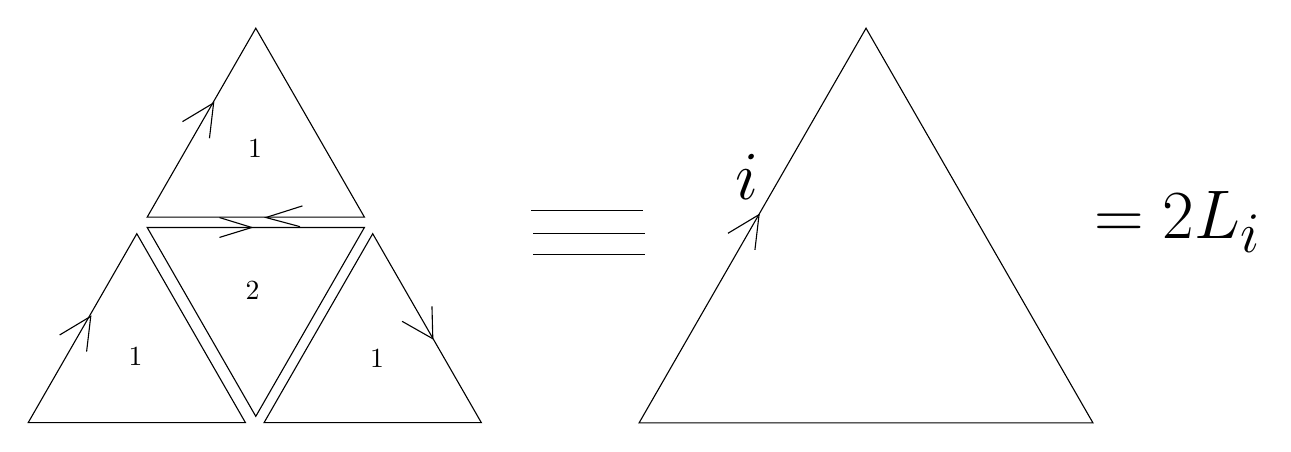
\begin{tikzpicture}[x=0.75pt,y=0.75pt,yscale=-1,xscale=1]
%uncomment if require: \path (0,300); %set diagram left start at 0, and has height of 300

%Shape: Triangle [id:dp40692481476808906] 
\draw   (144.32,20) -- (196.65,111) -- (92,111) -- cycle ;
%Shape: Triangle [id:dp6062532337301327] 
\draw   (144.32,207) -- (92,116) -- (196.65,116) -- cycle ;
%Shape: Triangle [id:dp3087361734769454] 
\draw   (200.65,119) -- (252.97,210) -- (148.32,210) -- cycle ;
%Shape: Triangle [id:dp4678656626426605] 
\draw   (87,119) -- (139.32,210) -- (34.68,210) -- cycle ;
%Straight Lines [id:da6851226797651961] 
\draw    (109,65) -- (124,56) -- (122,73) ;
%Straight Lines [id:da737765955033743] 
\draw    (49.8,167.8) -- (64.8,158.8) -- (62.8,175.8) ;
%Straight Lines [id:da8709391119480012] 
\draw    (126.8,111.2) -- (142.4,116) -- (126.8,120.8) ;
%Straight Lines [id:da1852761866859176] 
\draw    (166.8,105.6) -- (149.2,111.2) -- (165.6,115.6) ;
%Straight Lines [id:da30638262627497226] 
\draw    (229.2,154) -- (229.6,169.6) -- (214.8,161.2) ;

%Straight Lines [id:da8883030152871985] 
\draw    (277,108) -- (331,108) ;
%Straight Lines [id:da7208774874755355] 
\draw    (278,119) -- (332,119) ;
%Straight Lines [id:da6249118764365742] 
\draw    (278,129) -- (332,129) ;

%Shape: Triangle [id:dp03854775186272685] 
\draw   (438.33,20) -- (547.65,210.13) -- (329,210.13) -- cycle ;
%Straight Lines [id:da15276694786846567] 
\draw    (371.8,118.8) -- (386.8,109.8) -- (384.8,126.8) ;


% Text Node
\draw (139.4,72.4) node [anchor=north west][inner sep=0.75pt]    {$1$};
% Text Node
\draw (81.8,172.8) node [anchor=north west][inner sep=0.75pt]    {$1$};
% Text Node
\draw (198.2,173.6) node [anchor=north west][inner sep=0.75pt]    {$1$};
% Text Node
\draw (138.2,140.8) node [anchor=north west][inner sep=0.75pt]    {$2$};
% Text Node
\draw (547,97.4) node [anchor=north west][inner sep=0.75pt]  [font=\Huge]  {$=2L_i$};

% Text Node
\draw (374,79.4) node [anchor=north west][inner sep=0.75pt]  [font=\Huge]  {$i$};


\end{tikzpicture}


\end{center}
\end{solution}


\section{Problem 4}
\begin{solution}

Dimension analysis leads to $V=KR$. \newline
Each $d\theta$ sectors contributes equally.So, $dV=\frac{d\theta}{2\pi} KR$. We use this result in Figure-$2$ for sectors of variable radii given by $\frac{R}{\sqrt{2}} \sec{\theta}$, assuming square to be made of "4" right isosceles plates. So, 
\[V_o = 4 \int_{\frac{-\pi}{4}}^{\frac{\pi}{4}} \frac{d\theta}{2\pi} K \left(\frac{R}{\sqrt{2}} \sec{\theta}\right)\]
\[\implies V_0 = \frac{2\sqrt{2}}{\pi} KR \int_0^{\frac{\pi}{4}}\sec{\theta} d\theta\]
\[\implies V_0 = \frac{2\sqrt{2}}{\pi} KR \ln{\left(\sqrt{2}+1\right)}\]

\end{solution}


\section{Problem 5}
\begin{solution}
%% Figure 1
\begin{center}
    \tikzset{every picture/.style={line width=0.75pt}} %set default line width to 0.75pt        
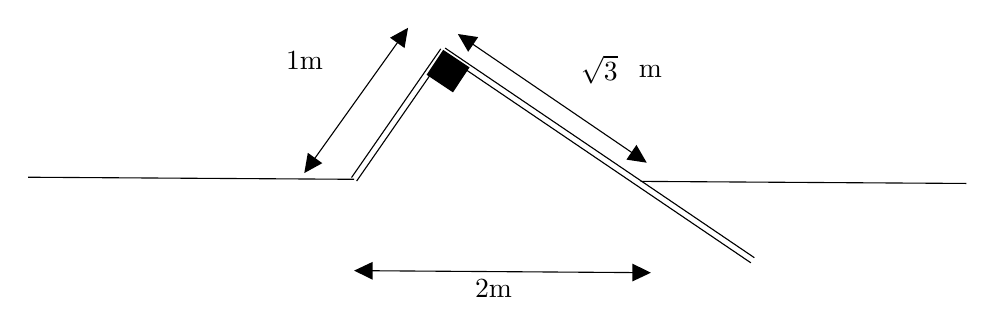
\begin{tikzpicture}[x=0.75pt,y=0.75pt,yscale=-1,xscale=1]
%uncomment if require: \path (0,300); %set diagram left start at 0, and has height of 300
%Straight Lines [id:da711233867243741] 
\draw    (100,118) -- (257,119) ;
%Straight Lines [id:da8574720198051322] 
\draw    (395,120) -- (508.99,120.73) -- (552,121) ;
%Straight Lines [id:da22926251509039042] 
\draw    (255.77,118.15) -- (298.77,56.15)(258.23,119.85) -- (301.23,57.85) ;
%Straight Lines [id:da448616977028955] 
\draw [fill={rgb, 255:red, 0; green, 0; blue, 0 }  ,fill opacity=1 ]   (448.16,159.24) -- (299.16,58.24)(449.84,156.76) -- (300.84,55.76) ;
%Shape: Rectangle [id:dp9153179604750035] 
\draw  [fill={rgb, 255:red, 0; green, 0; blue, 0 }  ,fill opacity=1 ] (300,57) -- (312.25,65.15) -- (304.56,76.73) -- (292.3,68.58) -- cycle ;
%Straight Lines [id:da8887552080956109] 
\draw    (260,163.02) -- (397,163.98) ;
\draw [shift={(400,164)}, rotate = 180.4] [fill={rgb, 255:red, 0; green, 0; blue, 0 }  ][line width=0.08]  [draw opacity=0] (8.93,-4.29) -- (0,0) -- (8.93,4.29) -- cycle    ;
\draw [shift={(257,163)}, rotate = 0.4] [fill={rgb, 255:red, 0; green, 0; blue, 0 }  ][line width=0.08]  [draw opacity=0] (8.93,-4.29) -- (0,0) -- (8.93,4.29) -- cycle    ;
%Straight Lines [id:da97162948128714] 
\draw    (234.74,113.56) -- (281.26,48.44) ;
\draw [shift={(283,46)}, rotate = 485.54] [fill={rgb, 255:red, 0; green, 0; blue, 0 }  ][line width=0.08]  [draw opacity=0] (8.93,-4.29) -- (0,0) -- (8.93,4.29) -- cycle    ;
\draw [shift={(233,116)}, rotate = 305.54] [fill={rgb, 255:red, 0; green, 0; blue, 0 }  ][line width=0.08]  [draw opacity=0] (8.93,-4.29) -- (0,0) -- (8.93,4.29) -- cycle    ;
%Straight Lines [id:da2997316618055039] 
\draw    (395.52,109.31) -- (309.48,50.69) ;
\draw [shift={(307,49)}, rotate = 394.27] [fill={rgb, 255:red, 0; green, 0; blue, 0 }  ][line width=0.08]  [draw opacity=0] (8.93,-4.29) -- (0,0) -- (8.93,4.29) -- cycle    ;
\draw [shift={(398,111)}, rotate = 214.27] [fill={rgb, 255:red, 0; green, 0; blue, 0 }  ][line width=0.08]  [draw opacity=0] (8.93,-4.29) -- (0,0) -- (8.93,4.29) -- cycle    ;
% Text Node
\draw (314,166) node [anchor=north west][inner sep=0.75pt]   [align=left] {2m};
% Text Node
\draw (223,56) node [anchor=north west][inner sep=0.75pt]   [align=left] {1m\\};
% Text Node
\draw (365,58) node [anchor=north west][inner sep=0.75pt]    {$\sqrt{3}$};
% Text Node
\draw (393,63) node [anchor=north west][inner sep=0.75pt]   [align=left] {m};
\end{tikzpicture}
\end{center}

%% Figure 2
\begin{center}
    

\tikzset{every picture/.style={line width=0.75pt}} %set default line width to 0.75pt        

\begin{tikzpicture}[x=0.75pt,y=0.75pt,yscale=-1,xscale=1]
%uncomment if require: \path (0,300); %set diagram left start at 0, and has height of 300

%Straight Lines [id:da711233867243741] 
\draw    (2,143.17) -- (230.71,144.63) ;
%Straight Lines [id:da8574720198051322] 
\draw    (431.74,146.08) -- (597.79,147.14) -- (660.45,147.54) ;
%Straight Lines [id:da22926251509039042] 
\draw [color={rgb, 255:red, 140; green, 14; blue, 252 }  ,draw opacity=1 ][fill={rgb, 255:red, 255; green, 0; blue, 0 }  ,fill opacity=1 ]   (229.48,143.77) -- (292.12,53.45)(231.94,145.48) -- (294.58,55.16) ;
%Shape: Arc [id:dp09390960457131636] 
\draw  [draw opacity=0] (231.35,146.08) .. controls (231.35,145.73) and (231.35,145.39) .. (231.35,145.04) .. controls (231.93,89.88) and (277.11,45.63) .. (332.27,46.21) .. controls (387.43,46.79) and (431.67,91.97) .. (431.1,147.13) .. controls (431.09,147.73) and (431.08,148.34) .. (431.06,148.94) -- (331.22,146.08) -- cycle ; \draw   (231.35,146.08) .. controls (231.35,145.73) and (231.35,145.39) .. (231.35,145.04) .. controls (231.93,89.88) and (277.11,45.63) .. (332.27,46.21) .. controls (387.43,46.79) and (431.67,91.97) .. (431.1,147.13) .. controls (431.09,147.73) and (431.08,148.34) .. (431.06,148.94) ;
%Straight Lines [id:da019158372781863164] 
\draw [color={rgb, 255:red, 255; green, 8; blue, 8 }  ,draw opacity=1 ]   (230.71,144.63) -- (230.71,79.62) ;
\draw [shift={(230.71,77.62)}, rotate = 450] [color={rgb, 255:red, 255; green, 8; blue, 8 }  ,draw opacity=1 ][line width=0.75]    (10.93,-3.29) .. controls (6.95,-1.4) and (3.31,-0.3) .. (0,0) .. controls (3.31,0.3) and (6.95,1.4) .. (10.93,3.29)   ;
%Straight Lines [id:da6400107435780602] 
\draw [color={rgb, 255:red, 246; green, 0; blue, 0 }  ,draw opacity=1 ]   (293.35,54.31) -- (346.86,31.78) ;
\draw [shift={(348.71,31)}, rotate = 517.1700000000001] [color={rgb, 255:red, 246; green, 0; blue, 0 }  ,draw opacity=1 ][line width=0.75]    (10.93,-3.29) .. controls (6.95,-1.4) and (3.31,-0.3) .. (0,0) .. controls (3.31,0.3) and (6.95,1.4) .. (10.93,3.29)   ;
%Straight Lines [id:da6946145063260911] 
\draw  [dash pattern={on 0.84pt off 2.51pt}]  (230.71,144.63) -- (431.74,146.08) ;
%Shape: Circle [id:dp8427051743011251] 
\draw  [fill={rgb, 255:red, 0; green, 0; blue, 0 }  ,fill opacity=1 ] (329.22,145.35) .. controls (329.22,144.25) and (330.12,143.35) .. (331.22,143.35) .. controls (332.33,143.35) and (333.22,144.25) .. (333.22,145.35) .. controls (333.22,146.46) and (332.33,147.35) .. (331.22,147.35) .. controls (330.12,147.35) and (329.22,146.46) .. (329.22,145.35) -- cycle ;
%Straight Lines [id:da27290473589018815] 
\draw  [dash pattern={on 4.5pt off 4.5pt}]  (293.35,54.31) -- (331.22,145.35) ;
%Straight Lines [id:da0371987429410201] 
\draw  [dash pattern={on 4.5pt off 4.5pt}]  (230.71,144.63) -- (329.22,145.35) ;
%Shape: Arc [id:dp6875478093811267] 
\draw  [draw opacity=0] (309.93,145.01) .. controls (309.83,144.38) and (309.78,143.73) .. (309.78,143.07) .. controls (309.78,137.03) and (314.08,132.14) .. (319.39,132.14) .. controls (321.29,132.14) and (323.06,132.76) .. (324.55,133.84) -- (319.39,143.07) -- cycle ; \draw   (309.93,145.01) .. controls (309.83,144.38) and (309.78,143.73) .. (309.78,143.07) .. controls (309.78,137.03) and (314.08,132.14) .. (319.39,132.14) .. controls (321.29,132.14) and (323.06,132.76) .. (324.55,133.84) ;
%Straight Lines [id:da22017865510269963] 
\draw    (236,159.06) -- (330,160.94) ;
\draw [shift={(333,161)}, rotate = 181.15] [fill={rgb, 255:red, 0; green, 0; blue, 0 }  ][line width=0.08]  [draw opacity=0] (8.93,-4.29) -- (0,0) -- (8.93,4.29) -- cycle    ;
\draw [shift={(233,159)}, rotate = 1.15] [fill={rgb, 255:red, 0; green, 0; blue, 0 }  ][line width=0.08]  [draw opacity=0] (8.93,-4.29) -- (0,0) -- (8.93,4.29) -- cycle    ;
%Straight Lines [id:da5564189152636927] 
\draw  [dash pattern={on 0.84pt off 2.51pt}]  (293.35,54.31) -- (404,56) ;
%Shape: Free Drawing [id:dp703247676082269] 
\draw  [color={rgb, 255:red, 0; green, 0; blue, 0 }  ][line width=0.75] [line join = round][line cap = round] (318,48) .. controls (318,51.33) and (318,61.33) .. (318,58) .. controls (318,54.33) and (318.56,50.62) .. (318,47) .. controls (317.78,45.6) and (314.37,42.74) .. (315,44) .. controls (316.97,47.94) and (319,48.69) .. (319,54) ;
%Shape: Free Drawing [id:dp2465244774746833] 
\draw  [color={rgb, 255:red, 0; green, 0; blue, 0 }  ][line width=0.75] [line join = round][line cap = round] (314,45) .. controls (319.59,45) and (317,56.13) .. (317,56) .. controls (317,52.65) and (317.5,49) .. (316,46) .. controls (315.94,45.87) and (315.24,41.76) .. (314,43) .. controls (313.59,43.41) and (316,47.37) .. (316,48) ;

% Text Node
\draw (287,117) node [anchor=north west][inner sep=0.75pt]    {$60^{\circ }$};
% Text Node
\draw (270,159) node [anchor=north west][inner sep=0.75pt]    {$1m$};
% Text Node
\draw (262.03,99.47) node [anchor=north west][inner sep=0.75pt]    {$1m$};
% Text Node
\draw (208,94) node [anchor=north west][inner sep=0.75pt]  [font=\Large]  {$v$};
% Text Node
\draw (306,11) node [anchor=north west][inner sep=0.75pt]  [font=\Large]  {$v$};
% Text Node
\draw (321.03,42.65) node [anchor=north west][inner sep=0.75pt]  [font=\small]  {$30^{\circ }$};


\end{tikzpicture}
\end{center}
\end{solution}
\section{Problem 6}
\begin{solution}
For a low resistivity fluid, consider a bunch of fluid elements forming a loop. As the fluid moves, the loop changes shape, expands/contacts, etc.\par
If the magnetic field through the loop changes, there is an electric field curl induced. But, that leads to the flow of current, which opposes the change in magnetic field. In the limit of very low resistivity, the magnetic field through the loop can not change. It stays a constant.\par
Now, let us consider two loops at $t=0$ in the fluid as shown.\par
\begin{center}
\tikzset{every picture/.style={line width=0.75pt}} %set default line width to 0.75pt

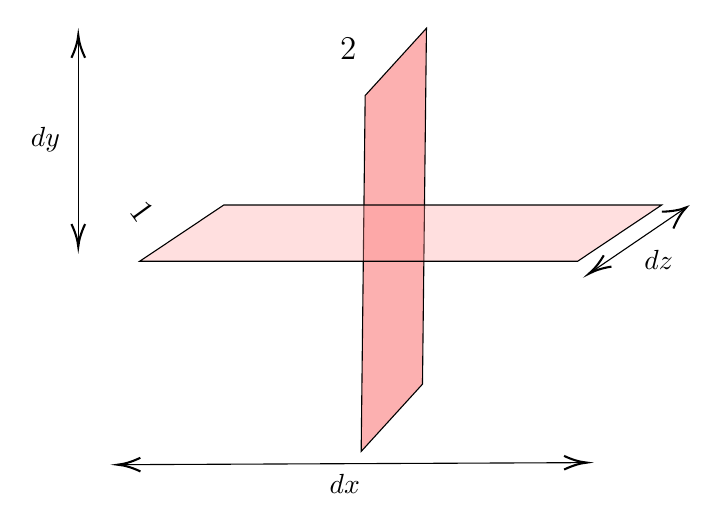
\begin{tikzpicture}[x=0.75pt,y=0.75pt,yscale=-1,xscale=1]
%uncomment if require: \path (0,300); %set diagram left start at 0, and has height of 300

%Flowchart: Data [id:dp7035880816369227] 
\draw  [fill={rgb, 255:red, 246; green, 0; blue, 0 }  ,fill opacity=0.31 ] (219.34,41.25) -- (248.87,8.82) -- (246.95,180.3) -- (217.41,212.73) -- cycle ;
%Shape: Rectangle [id:dp04887569784950463] 
\draw  [fill={rgb, 255:red, 255; green, 149; blue, 149 }  ,fill opacity=0.3 ] (151.2,94) -- (362.19,94) -- (321.68,121.11) -- (110.69,121.11) -- cycle ;
%Straight Lines [id:da09905766820455364] 
\draw    (372.45,96.23) -- (328.76,125.98) ;
\draw [shift={(327.11,127.11)}, rotate = 325.75] [color={rgb, 255:red, 0; green, 0; blue, 0 }  ][line width=0.75]    (10.93,-3.29) .. controls (6.95,-1.4) and (3.31,-0.3) .. (0,0) .. controls (3.31,0.3) and (6.95,1.4) .. (10.93,3.29)   ;
\draw [shift={(374.11,95.11)}, rotate = 145.75] [color={rgb, 255:red, 0; green, 0; blue, 0 }  ][line width=0.75]    (10.93,-4.9) .. controls (6.95,-2.3) and (3.31,-0.67) .. (0,0) .. controls (3.31,0.67) and (6.95,2.3) .. (10.93,4.9)   ;
%Straight Lines [id:da7533540101666225] 
\draw    (81.11,112.11) -- (81.11,14.11) ;
\draw [shift={(81.11,12.11)}, rotate = 450] [color={rgb, 255:red, 0; green, 0; blue, 0 }  ][line width=0.75]    (10.93,-3.29) .. controls (6.95,-1.4) and (3.31,-0.3) .. (0,0) .. controls (3.31,0.3) and (6.95,1.4) .. (10.93,3.29)   ;
\draw [shift={(81.11,114.11)}, rotate = 270] [color={rgb, 255:red, 0; green, 0; blue, 0 }  ][line width=0.75]    (10.93,-3.29) .. controls (6.95,-1.4) and (3.31,-0.3) .. (0,0) .. controls (3.31,0.3) and (6.95,1.4) .. (10.93,3.29)   ;
%Straight Lines [id:da901491630243338] 
\draw    (102.11,219.1) -- (324.11,218.12) ;
\draw [shift={(326.11,218.11)}, rotate = 539.75] [color={rgb, 255:red, 0; green, 0; blue, 0 }  ][line width=0.75]    (10.93,-3.29) .. controls (6.95,-1.4) and (3.31,-0.3) .. (0,0) .. controls (3.31,0.3) and (6.95,1.4) .. (10.93,3.29)   ;
\draw [shift={(100.11,219.11)}, rotate = 359.75] [color={rgb, 255:red, 0; green, 0; blue, 0 }  ][line width=0.75]    (10.93,-3.29) .. controls (6.95,-1.4) and (3.31,-0.3) .. (0,0) .. controls (3.31,0.3) and (6.95,1.4) .. (10.93,3.29)   ;

% Text Node
\draw (113.8,89.28) node [anchor=north west][inner sep=0.75pt]  [font=\large,rotate=-53.78]  {$1$};
% Text Node
\draw (201,222.4) node [anchor=north west][inner sep=0.75pt]    {$dx$};
% Text Node
\draw (57,55.4) node [anchor=north west][inner sep=0.75pt]    {$dy$};
% Text Node
\draw (352.61,114.51) node [anchor=north west][inner sep=0.75pt]    {$dz$};
% Text Node
\draw (206,12.4) node [anchor=north west][inner sep=0.75pt]  [font=\large]  {$2$};

\end{tikzpicture}  
\end{center}
The loop $1$ has flux $B_0 dx dz$ through it, Whereas loop $2$ has flux $0$ through it.\par
Now, let us look at where these loops will end up after a time $t$ and how they will look.\par
The loops are moved ahead by $vt$, and oriented as shown below: \par
\begin{center}
\tikzset{every picture/.style={line width=0.75pt}} %set default line width to 0.75pt

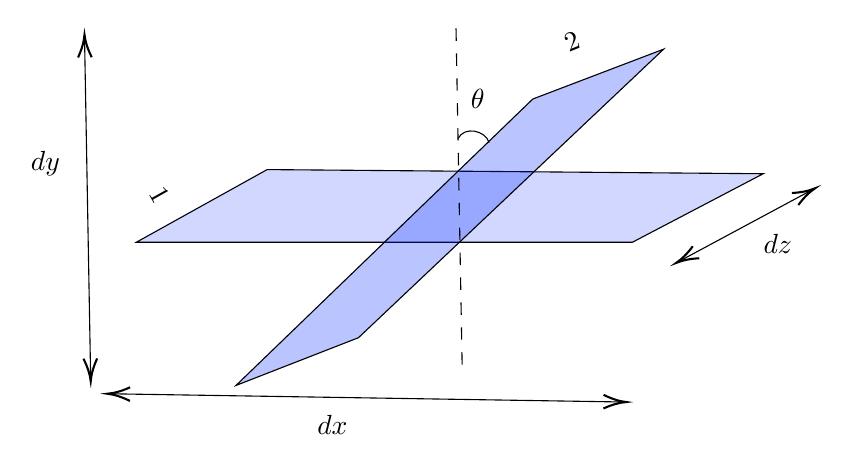
\begin{tikzpicture}[x=0.75pt,y=0.75pt,yscale=-1,xscale=1]
%uncomment if require: \path (0,300); %set diagram left start at 0, and has height of 300

%Shape: Polygon [id:ds916886588727925] 
\draw  [fill={rgb, 255:red, 0; green, 31; blue, 255 }  ,fill opacity=0.18 ] (204.11,116.47) -- (443.11,118.47) -- (380.11,151.47) -- (141.11,151.47) -- cycle ;
%Shape: Polygon [id:ds05642300854837812] 
\draw  [fill={rgb, 255:red, 0; green, 40; blue, 255 }  ,fill opacity=0.27 ] (395.11,58.47) -- (332.11,82.47) -- (189.11,220.47) -- (248.11,197.47) -- cycle ;
%Straight Lines [id:da3195531099085156] 
\draw  [dash pattern={on 4.5pt off 4.5pt}]  (295.11,48.47) -- (298.11,213.47) ;
%Curve Lines [id:da3017736924368517] 
\draw    (311.11,103.47) .. controls (309.11,97.47) and (299.11,95.47) .. (296.11,101.47) ;
%Straight Lines [id:da5840092338247029] 
\draw    (402.87,160.52) -- (466.35,126.42) ;
\draw [shift={(468.11,125.47)}, rotate = 511.75] [color={rgb, 255:red, 0; green, 0; blue, 0 }  ][line width=0.75]    (10.93,-3.29) .. controls (6.95,-1.4) and (3.31,-0.3) .. (0,0) .. controls (3.31,0.3) and (6.95,1.4) .. (10.93,3.29)   ;
\draw [shift={(401.11,161.47)}, rotate = 331.75] [color={rgb, 255:red, 0; green, 0; blue, 0 }  ][line width=0.75]    (10.93,-3.29) .. controls (6.95,-1.4) and (3.31,-0.3) .. (0,0) .. controls (3.31,0.3) and (6.95,1.4) .. (10.93,3.29)   ;
%Straight Lines [id:da20333438746325694] 
\draw    (119.07,216.47) -- (116.14,53.47) ;
\draw [shift={(116.11,51.47)}, rotate = 448.97] [color={rgb, 255:red, 0; green, 0; blue, 0 }  ][line width=0.75]    (10.93,-3.29) .. controls (6.95,-1.4) and (3.31,-0.3) .. (0,0) .. controls (3.31,0.3) and (6.95,1.4) .. (10.93,3.29)   ;
\draw [shift={(119.11,218.47)}, rotate = 268.97] [color={rgb, 255:red, 0; green, 0; blue, 0 }  ][line width=0.75]    (10.93,-3.29) .. controls (6.95,-1.4) and (3.31,-0.3) .. (0,0) .. controls (3.31,0.3) and (6.95,1.4) .. (10.93,3.29)   ;
%Straight Lines [id:da6448390957358343] 
\draw    (129.11,224.5) -- (375.11,228.44) ;
\draw [shift={(377.11,228.47)}, rotate = 180.92] [color={rgb, 255:red, 0; green, 0; blue, 0 }  ][line width=0.75]    (10.93,-3.29) .. controls (6.95,-1.4) and (3.31,-0.3) .. (0,0) .. controls (3.31,0.3) and (6.95,1.4) .. (10.93,3.29)   ;
\draw [shift={(127.11,224.47)}, rotate = 0.92] [color={rgb, 255:red, 0; green, 0; blue, 0 }  ][line width=0.75]    (10.93,-3.29) .. controls (6.95,-1.4) and (3.31,-0.3) .. (0,0) .. controls (3.31,0.3) and (6.95,1.4) .. (10.93,3.29)   ;

% Text Node
\draw (301,76.4) node [anchor=north west][inner sep=0.75pt]    {$\theta $};
% Text Node
\draw (154.71,122.06) node [anchor=north west][inner sep=0.75pt]  [rotate=-60.82]  {$1$};
% Text Node
\draw (344.59,51.2) node [anchor=north west][inner sep=0.75pt]  [rotate=-338]  {$2$};
% Text Node
\draw (442,146.4) node [anchor=north west][inner sep=0.75pt]    {$dz$};
% Text Node
\draw (89,106.4) node [anchor=north west][inner sep=0.75pt]    {$dy$};
% Text Node
\draw (227,233.4) node [anchor=north west][inner sep=0.75pt]    {$dx$};

\end{tikzpicture}
\end{center}
The flux through loop $2$ is still $0$. The flux through loop 1 is still $B_0 dx dz$. \par 
Thus, the magnetic field looks as shown:

\end{solution}
\section{Problem 7}
\begin{solution}
Light rays going toward a focus of the hyperbola, upon reflection, change their paths so as to go through the other focus. Following the light path, we see that no rays can get to the point $O_1$.
    \begin{center}
    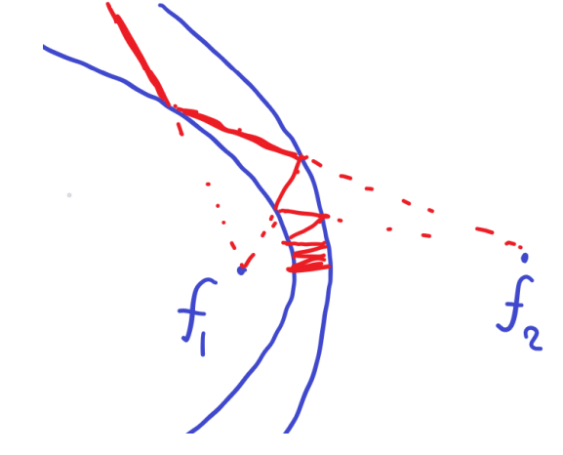
\includegraphics[width=0.5\textwidth]{okkkkk.png}    
    \end{center}
\end{solution}
\section{Problem 8}
\begin{solution}

\end{solution}
\section{Problem 9}
\begin{solution}
Since $R<<d$, $\vec{E}$ everywhere except near hemisphere will be:
$$
\boxed{
    |\vec{E}|=\frac{V<em>0}{d}
}
$$

In uniform electric field grounded sphere gets polarised with dipole moment:


%Insert Fig 2 here

$$
\boxed{
    | \vec{p} |=\frac{4}{3} \pi R^3 3\epsilon</em>{0} \vec{E<em>0}
}
$$


So, surface charge density will be:


%Insert Fig 3 here


$$\boxed{
\sigma = -3\epsilon</em>{0} E<em>0 cos\theta
}
$$


%Insert Fig 4 here


$$\boxed{\vec{E} = \frac{\sigma}{\epsilon</em>{0}}=-3E_0 cos\theta \hat{r}} $$

Ohms law:

$$\vec{J}=\sigma \vec{E}$$
$$\vec{J} = -3E_0 \cos \theta \sigma \hat{r}$$
$$\ \ \ = -3\sigma \cos\theta\frac{V_0}{d} \hat{r}$$

So, total current flowing inside hemisphere will be 
$$ I= \int \vec{J} \cdot d \vec{A}$$
$$\ \ \ = \int_0^{\frac{\pi}{2}} 3\sigma \cos\theta\frac{V_0}{d} \cdot 2\pi R \sin \theta R d \theta$$

$$\boxed{\text{Hence, Answer=} \frac{3\pi R^2 \sigma V_0}{d}}$$
\end{solution}

\section{Problem 10}
\begin{solution}

Let's analyse the magic wand at an arbitrary distance $x$ from the left end, where $0 \leq x \leq l$

Infinitesimal resistance is \[dR = \frac{\rho}{\pi \left(R_0 + r {\sin{\theta}}^2 \frac{2 \pi x}{a} \right)} dl = \frac{\rho dx}{\pi R_{0}^2 \left( 1 + \frac{r}{R_0} \sin^2 \frac{2 \pi x}{a} \right)}\] 
\[\approx \frac{\rho dx}{\pi R_{0}^{2} \left( 1 + \frac{2r}{R_0} \sin^2 \frac{2 \pi x}{a} \right)}\]
Bionomial approximation gives \[R \approx \frac{\rho dx}{\pi R_{0}^{2}} \left( 1 - \frac{2r}{R_0} \sin^2 \frac{2 \pi x}{a} \right) = \frac{\rho dx}{\pi R_{0}^{2}} \left[ 1 - \frac{r}{R_0} \left( 1 - \cos \frac{4\pi x}{a} \right) \right] = \frac{\rho dx}{\pi R_{0}^2} \left( 1 - \frac{r}{R_0} + \frac{r}{R_0} \cos \frac{4 \pi x}{a} \right)\]

Now, we integrate $dR$ over whole wand with limits from $0$ to $l$
\[R = \int_{0}^{l} \frac{\rho dx}{\pi R_{0}^2} \left( 1 - \frac{r}{R_0} + \frac{r}{R_0} \cos \frac{4 \pi x}{a} \right)\]
\[= \frac{\rho dx}{\pi R_{0}^2} \left[ \left( 1 - \frac{r}{R_0} \right) x \right]^{l}_{0} + \left[ \frac{ar}{4 \pi R_0} \sin \frac{4 \pi x}{a} \right]^{l}_{0} = \frac{\rho l}{\pi R_{0}^2} \left( 1 - \frac{r}{R_0} \right)\]
Hence, the resistance is \[\boxed{R = \frac{\rho l}{\pi R_{0}^2} \left( 1 - \frac{r}{R_0} \right)}\]
\end{solution}



\end{document}